\documentclass{../../../fal_assignment}
\graphicspath{ {../../../} }

\usepackage{amsmath}
\usepackage{enumitem}
\setlist{nosep} % Make enumerate / itemize lists more closely spaced
\usepackage[T1]{fontenc} % http://tex.stackexchange.com/a/17858
\usepackage{url}
\usepackage{todonotes}
\usepackage{algpseudocode}
\usepackage{listings}
\lstset{
	basicstyle=\ttfamily,
	frame=single,
	showstringspaces=false
}
\lstset{
	commentstyle=\ttfamily\textit,
	keywordstyle=\ttfamily\textbf,
	stringstyle=\ttfamily,
	rulecolor=\color{black}
}
\lstset{language=[Sharp]C}

\title{Worksheet 7: Recursion}
\author{Dr Ed Powley}
\module{COMP110}
\version{3.0}

\begin{document}

\maketitle
\marginpicture{flavour_pic}{
    A screenshot from Factorio, showing a successful rocket launch.
}

\section*{Introduction}

\textbf{Factorio} is a game in which players build factories to mine resources, assemble complex products from simpler ones, and ultimately build and launch a rocket into space.
In this worksheet, you will implement a tool which calculates the amount of raw resources required to assemble a given product.

Many products in Factorio can be crafted within the player's inventory according to a \textbf{recipe}.
The recipe specifies the materials it uses\footnote{Note for experienced Factorio players:
	in this worksheet we assume that every recipe crafts 1 product. Recipes which usually craft multiple products are divided accordingly.
	For example, rather than 2 copper cable requiring 1 copper plate and 0.5 seconds, we say that 1 copper cable requires 0.5 copper plates and 0.25 seconds.}
and the time it takes.
The exception is \textbf{raw materials}, which cannot be crafted by the player and instead have to be obtained from the world\footnote{Note for experienced Factorio players:
	I consider ``raw materials'' to be anything which cannot be crafted in the player's inventory.
	For example mined resources, smelting, recipes involving fluids, and certain products such as engine units.}.

For example, the \emph{automation-science-pack} requires 1 \emph{copper-plate} and 1 \emph{iron-gear-wheel}, and takes 5 seconds.
In turn, one \emph{iron-gear-wheel} requires 2 \emph{iron-plate} and takes 0.5 seconds.
This means, in total, the \emph{automation-science-pack} takes 1 \emph{copper-plate}, 2 \emph{iron-plate} and 5.5 seconds.
Note that \emph{copper-plate} and \emph{iron-plate} are raw materials.

Recipes encountered later in the game are much more complex, requiring many more intermediate products.
For example \emph{spidertron} (a vehicle that becomes available late in the game)
requires 7 different types of raw materials, and up to 6 stages of intermediate products between raw materials and the final product.

Note that this worksheet is using Factorio as an example, but you are \textbf{not} required to purchase or play the game.
Indeed, for time management reasons, you are actively discouraged from playing Factorio when assignment deadlines are present.

To complete this worksheet, \textbf{fork} the skeleton project and \textbf{open} the solution file in Visual Studio.
\textbf{Implement} the following methods of the \lstinline{Calculator} class:

\subsection*{\lstinline{GetTotalAssemblyTimeForProduct()}}

This method should return the total time (in seconds) to craft the given product from raw materials.
For example,
\begin{lstlisting}
GetTotalAssemblyTimeForProduct("automation-science-pack")
\end{lstlisting}
should return \lstinline{5.5} as explained above. 
If the given product is itself a raw material, this function should return \lstinline{0}.

\subsection*{\lstinline{GetRawMaterialsForProduct()}}

This method should return the names and quantities of the raw materials required to craft the given product.
These are returned as a dictionary mapping strings to quantities.
For example,
\begin{lstlisting}
GetRawMaterialsForProduct("automation-science-pack")
\end{lstlisting}
should return
\begin{lstlisting}
{
	["copper-plate"] = 1,
	["iron-plate"] = 2
}
\end{lstlisting}

If the given product is itself a raw material, this function should return a dictionary with a single entry for that product with a quantity of 1.
For example,
\begin{lstlisting}
GetRawMaterialsForProduct("iron-plate")
\end{lstlisting}
should return
\begin{lstlisting}
	{
		["iron-plate"] = 1
	}
\end{lstlisting}

\subsection*{Stretch goal}

For extra credit, implement a function which displays a breakdown of the intermediate products and raw materials for a given product.
It should output the information as an indented list, like so:

\begin{center}
	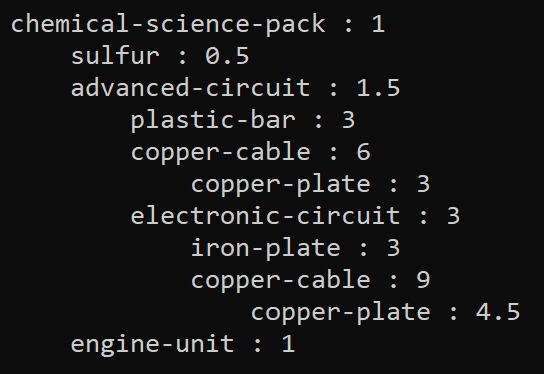
\includegraphics[width=0.6\textwidth]{stretch-goal}
\end{center}

For \emph{extra} extra credit, implement a function to display this information in a graphical format.
You may use external general-purpose libraries or tools (or even Unity) to display the information,
however you may \textbf{not} use any code from existing tools developed by the Factorio player community.

\subsection*{Navigating the skeleton project}

The skeleton project contains a file \texttt{Program.cs}, which you may find useful when testing your code.
There is also a unit test project which defines a series of tests using the MSTest framework;
these can be run locally within Visual Studio.

The provided \lstinline{Recipes} class loads a database of Factorio recipes, and provides the following useful methods:
\begin{itemize}
	\item \lstinline{IsRawMaterial()} determines whether the given product is considered a raw material.
	\item \lstinline{FindIngredientsForProduct()} returns the ingredients for a given product, as a dictionary
		whose keys are product names and whose values are quantities.
		If the product is a raw material, an error will be raised.
    \item \lstinline{FindAssemblyTimeForProduct()} returns the time in seconds to craft a given product.
		If the product is a raw material, an error will be raised.
\end{itemize}

\section*{Submission instructions}

Begin by \textbf{forking} the GitHub repository at the following URL:

\url{https://github.falmouth.ac.uk/Games-Academy/comp110-ws-recursion}

Edit \texttt{Calculator.cs}, implementing the required functions.
When you have finished, open a \textbf{pull request}.

\textbf{Do not move or rename \texttt{Calculator.cs}, and do not edit or delete any of the other files in the repository except for \texttt{Program.cs}}.
Doing so will interfere with the automated testing scripts used to check your submission for correctness,
and as a result may lead to you losing marks.

Upload all material to the git server and open a pull request by the deadline listed on LearningSpace.

\section*{Additional information}

A video is provided on LearningSpace which explains the worksheet in more detail and provides useful additional information.

\section*{Marking criteria}

Remember that \textbf{it is better to submit incomplete work than to submit nothing at all}.

Your work will be marked according to the following criteria:
\begin{itemize}
	\item \textbf{Functional coherence}. Is your implementation correct?
		Your code will be run through the unit tests to verify that it gives the correct results for a sample of input values.
	\item \textbf{Sophistication}. Have you made use of appropriate code structures and data structures?
		Note the emphasis is on \textbf{appropriate}; extra credit will \textbf{not} be given for unnecessarily complex solutions.
		However extra credit \textbf{will} be given for solutions that allow for efficient code reuse between functions,
		for example using iterator functions and/or LINQ.
	\item \textbf{Maintainability}. Is your code well commented? Are your identifier names appropriate and descriptive?
		Have you adhered to appropriate coding standards?
	\item \textbf{Stretch goal}. Have the stretch goals been completed? Partial credit will be given for partial attempts,
		and extra credit for particularly high-quality work.
\end{itemize}

\end{document}
